% --------------------------------------
% Master's Thesis Title Page
% LaTeX Template
% Version 1.0 (23/05/14)
% Thanks to Magnus Marthinsen, this thesis and template is made available for Master studentes at HVL Joint SE program (01.03.2021)
%---------------------------------------

%----------------------------------------------------------------------------------------
%	PACKAGES AND OTHER DOCUMENT CONFIGURATIONS
%----------------------------------------------------------------------------------------
\documentclass[a4paper]{report}
\usepackage{graphicx} % Required for box manipulation
\usepackage{helvet}
\usepackage{subfig}
\usepackage[utf8]{inputenc}
%\usepackage{natbib}
\usepackage[USenglish]{babel}
\usepackage[useregional]{datetime2}
\usepackage{pgfgantt}
\usepackage{listings}
\usepackage{wrapfig}
\usepackage{setspace}
\usepackage{parskip} % Used to create spaces between paragraphs
\usepackage{dirtytalk} % quotes by talk
\usepackage[hidelinks]{hyperref}
% \usepackage[acronym, toc]{glossaries}  % Used to add a wordlist/glossaries
\usepackage{mathtools}
\usepackage{amsfonts}
\usepackage{color, colortbl}
\usepackage{booktabs}
\usepackage{float}
\usepackage{csquotes}

%BIB by Adrian
\usepackage[backend=biber,style=numeric, urldate=long]{biblatex}
% See the references.bib file. Most Bibtex bibliographies in Computer Science can be found from dblp.org
\addbibresource{report.bib}



% Glossary/wordlist
% \makeglossaries
% \input{glossaries.tex}

\begin{document}

%
% COLORS USED THROUGH THE REPORT
%
\definecolor{kb_red}{RGB}{96,2,4}
\definecolor{light_gray}{RGB}{160,160,160}
\definecolor{med_gray}{RGB}{96,94,94}
\definecolor{black}{RGB}{0,0,0}
\definecolor{white}{RGB}{155,155,155}
\definecolor{light_green}{RGB}{208,240,192}
\definecolor{light_red}{RGB}{255,204,203}

% CODE STYLE
\definecolor{javared}{rgb}{0.6,0,0} % for strings
\definecolor{javagreen}{rgb}{0.25,0.5,0.35} % comments
\definecolor{javapurple}{rgb}{0.5,0,0.35} % keywords
\definecolor{javadocblue}{rgb}{0.25,0.35,0.75} % javadoc

\makeatletter
\lst@Key{matchrangestart}{f}{\lstKV@SetIf{#1}\lst@ifmatchrangestart}
\def\lst@SkipToFirst{%
    \lst@ifmatchrangestart\c@lstnumber=\numexpr-1+\lst@firstline\fi
    \ifnum \lst@lineno<\lst@firstline
        \def\lst@next{\lst@BeginDropInput\lst@Pmode
        \lst@Let{13}\lst@MSkipToFirst
        \lst@Let{10}\lst@MSkipToFirst}%
        \expandafter\lst@next
    \else
        \expandafter\lst@BOLGobble
    \fi}
\makeatother

\lstset{language=Java,
basicstyle=\footnotesize,
keywordstyle=\color{javapurple}\bfseries,
stringstyle=\color{javared},
commentstyle=\color{javagreen},
morecomment=[s][\color{javadocblue}]{/**}{*/},
numbers=left,
captionpos=b,
frame=single,
breakatwhitespace=false,
breaklines=true,
numberstyle=\tiny\color{black},
stepnumber=1,
numbersep=10pt,
tabsize=2,
showspaces=false,
showstringspaces=false,
matchrangestart=t}

%----------------------------------------------------------------------------------------
%	TITLE PAGE
%----------------------------------------------------------------------------------------

\newcommand*{\titlePage}{\begingroup % Create the command for including the title page in the document
\fontfamily{phv}\selectfont
\centering % Center all text
\DTMlangsetup[en-US]{showdayofmonth=false}

%----------------------------------------------------------------------------------------
%	TITLE SECTION
%----------------------------------------------------------------------------------------

\vspace{200pt}
{\Huge VR viewer} \\ % Title
\vspace{5pt}

{\Large \textsl{}} % Subtitle or further description
\vspace{50pt}

%----------------------------------------------------------------------------------------
%	AUTHOR SECTION
%----------------------------------------------------------------------------------------

\LARGE{\textbf{Tobias Eilertsen}}\\ % Author name

\vfill % Whitespace between the author name and the school

%----------------------------------------------------------------------------------------
%	DESCRIPTION AND DATE SECTION
%----------------------------------------------------------------------------------------


{\Large \textbf{Master's thesis in Software Engineering at} \\
\vspace{10pt}
Department of Computer science, Electrical engineering and Mathematical sciences, \\
Western Norway University of Applied Sciences \\
\vspace{10pt}
Department of  Informatics, \\
University of Bergen \\}
\vspace{10pt}
{\large \today} % Month and year published

%----------------------------------------------------------------------------------------
%	LOGO SECTION
%----------------------------------------------------------------------------------------

\vfill % Whitespace between the school and the publisher logo


\begin{figure}[h!]
	\captionsetup[subfigure]{labelformat=empty}
	\subfloat[][]{
\includegraphics[height=70pt]{images/logos/hvl_logo_engelsk.pdf}}
	\hfill
	\subfloat[][]{
\includegraphics[height=70pt]{images/logos/uib-logo.eps}}
\end{figure}


\endgroup}

\titlePage
\pagebreak

\section*{Abstract}
During the planning of a surgery in orthopedics, the surgeons will use CT scans and sometimes 3D printing to analyze the fracture and help prepare for the surgery. By using Virtual Reality technology, the data can be visualized in 3D in a more immersive way, potentially improving the preparation phase by increasing the anatomical understanding or removing the need for 3D printing.

% \section*{Acknowledgements}
% First and foremost, I would like to thank

% \listoftables

% \printglossary[nonumberlist]
% \printglossary[type=\acronymtype, nonumberlist]

\chapter{Introduction}
This thesis is written as part of the University of Bergen and Western University of Applied Sciences master programme in software engineering. The project is a collaboration with Helse Vest IKT and orthopedic surgeons at Haukeland University Hospital.


\section{Context and Approach}
A CT scan is often performed when a hospital receives an injured patient considered for orthopedic surgery. The CT scan is displayed as 2D images or as a 3D model. The model allows the surgeons to better plan the surgery by understanding the anatomy of the fracture.
If a surgeon has a good understanding of the anatomy related to the fracture,
the surgery has less risk of complications or could require fewer resources.

\section{Problem Description}
Visualizing the model in 2D limits the understanding of the fracture because of the lack of scale and depth. The problem applies to both 2D images and 3D models rendered in 3D.
A considered solution is visualizing the model in Augmented Reality or Virtual Reality to give medical personnel a good understanding of the problem area.
VR has multiple potential benefits, and the surgery planning process can use some of these. As the users are already looking at 3D models on 2D screens, visualizing in VR could improve the surgeon's overview and patient safety. The entire planning process could also be more effective by removing or reducing the need for 3D printed models, especially in cases with limited time. Therefore the possible research questions are as follows:

Can VR technology improve surgery planning by

1: a better understanding giving a better success rate.

2: using less resources or time compared to 3D printing with the same benefits

\section{Methodology}

The project should include a VR prototype of a standard where it is
user friendly enough to test with non-technical subjects and with functionality
that is comparable to the use cases of a printed model.
The prototype is tested on medical personnel to measure any benefits on anatomical understanding and how it affects surgery planning and effectiveness.
The application should be available for further development and study.

Firstly, a prototype VR viewer will be created with the help of related
open-source frameworks/software and guidance from both orthopedic surgeons and
developers with experience in medical technology.

In order to answer the research question, it is necessary to measure the
performance of the final application. This thesis will use qualitative methods
by interviewing related personnel to investigate the performance, including
anatomical understanding, cooperation, and the effectiveness of the planning
process.
The performance will also be put in context to the existing solutions, possibly
by making a direct comparison by using a 3D model, printed model, and VR viewer
on the same case.

\chapter{Background}\label{Background}
This chapter will present some of the knowledge that our research is built upon. 

\section{orthopedic surgery}

Orthopedic surgery is surgery involving the musculoskeletal system. Cases range from trauma surgery, where high impact forces cause injuries to infections and tumors\cite{manual ortho}.

Orthopedic surgeons do both elective (planned) and urgent surgery. In elective surgery, the surgeons will have days or weeks to plan out the surgery. A team of usually two surgeons will plan the surgery together.
A surgeon will diagnose the patient from the following features: history, clinical examination, medical imaging, and any special investigations. History includes the patient's complaint and any previous injuries. Clinical investigation means examining the sources of the symptoms and the body as a whole. Medical imaging, including ultrasound, CT, and MRI, gives the surgeons a detailed insight into bones or soft tissue structures.

This research is based on elective surgeries on trauma or fractures where the surgeons plan out the surgery with different tools.


\subsection{Visualisation of medical imaging}

The output of both CT and MRI scans is a three-dimensional scan. The output is typically represented as slices, where a slice is a 2D picture repeating along an angle. The pixel at coordinate \emph{(x, y)} at slice number \emph{z} represent the absorption at the point \emph{(x, y, z)}\cite{chougule_conversions_2013}.
Each pixel in a slice represents a voxel in a volume, and all the slices combined make up volumetric data or a three-dimensional point cloud\cite{chougule_conversions_2013}.
The slice thickness of a slice can be below 1 mm, giving a high-resolution scan where a single point is less than one cubic millimeter\cite{hamblen_outline_2010}.

When rendering a 2D image, the volume must be projected to two-dimensional space. The values in a single slice can be used to view the intersection at a specific slice number. A line of values along all the slices can be used to view the intersection at another plane.
All slices can be combined to show either the average or the maximum intensity\cite{fishman_volume_2006}.
The values are converted to greyscale by mapping ranges of values to greyscale pixels. This mapping function determines the brightness and contrast of the final image.


\begin{figure}[h!]
    \centering
	\subfloat[][]{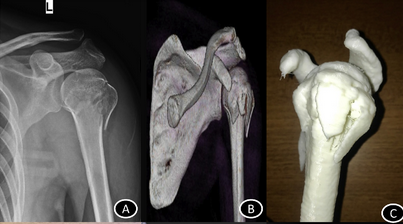
\includegraphics[height=120pt]{images/ctToPrint.png}}
	\hfill
  \caption{Humeral (upper arm) fracture}
  \small
    A fracture from initial scan to finished print. (A) preoperative X-ray; (B) 3D model; (C) 3D printed model.
~Image from study on virtual preoperative planning~\cite{mishra_virtual_2019}
\end{figure}


\chapter{Design and Implementation}\label{Design and Implementation}

\section{Demonstration}\label{demonstration}
Short video demo: \url{https://drive.google.com/file/d/18STcROOth1cwyF2sgASgVg7g4b8PSL88/view?usp=sharing}

\section{Development methods}

\subsection{Research Method}
The research question is solved by developing an application, and evaluating the application with respect to the research questions. Qualitative is used, because of a low test user amount.

The largest part of the study is developing the application that fills the need of viewing CT data. This is accomplished by uncovering user needs with interviews and user testing. When the application meets minimum specifications, an evaluation if performed. 

The evaluation at the end of the project aims to answer both research questions. The evaluation is done in the following way:
The test users try the application on their own in a relevant scenario.
The users respond to a semi-structured interview. The questions are specific towards both research questions.

The responses are gathered and used to answer the questions.

\subsection{Iterative Development}

The application is developed using iterative development and elements from Design Thinking and Scrum.

Scrum was used to cooperate effectively with the team and increase the development speed. The team had regular meetings and this fits well with the sprints used in scrum and the surgeon on the team was a natural product owner.
The team had regular biweekly meetings with a demonstration, sprint retrospective, and sprint planning. The Sprint meeting was a valuable way of sharing interdisciplinary information and getting feedback from medical experts. Sprint retrospective and daily scrum was not relevant as only one person worked full time on the project.
After the biweekly demo, the sprint backlog was updated with tasks prioritized by value. The value is determined by the time needed to implement compared to how important the functionality is to the medical personnel. Any tasks or ideas remaining are stored in the product backlog and considered for the next sprint.
The frequent Scrum demonstrations worked really well with VR development, as the different features are hard to understand without trying the application. Fast prototypes are important to cooperate efficiently when the product owner or test users have a limited understanding of the technology.

Design thinking was loosely used because the medical domain and user needs was difficult to understand. I specifically used the ideate, prototype and test pattern to develop the application
The application demos served as smaller user testing sessions. The medical personnel in the team would try out the application and any new features and give feedback and ideas during testing. User testing would often lead to new ideas. Optimally the test subjects should have been personnel outside the project without any bias, but busy schedules and COVID restrictions limited this.

\section{Project overview}\label{CodeStructure}

\section{Design}

\subsection{Design goals}

The goal of the application design is as follows:
give a good understanding of what the fracture looks like (bruddlinje og mindre biter)
Ease of use for non technical personnel
Be able to cooperate in smaller teams - multiplayer


\subsection{VR interface}

To make the VR interface easy to use, I focused primarily on familiarity with current tools and a simple design.
I used MicroDICOM\cite{MicroDICOM} as a reference for a familiar tool.
Familiarity with current tools means taking interactions from programs such as CT viewers and adopting the same interactions to VR to make it recognizable and consistent to the user. An example of this is navigating a menu in VR the same way one would navigate a menu with a pc mouse.
 All unnecessary interactions and information is removed to allow new users with little VR experience to start using the program quickly. The goal is to make the experience less overwhelming and lower the skill required to use the viewer effectively.

\subsubsection{Learning process}
A video game style tutorial was considered, where the user would go through tasks with hints or descriptions of the features in the application. However, this was not implemented as early testing revealed users were learning the controls quickly.

Every button has a description displayed as text above the button to remind the user of the keybindings. An image can optionally be displayed, showing the user the keybindings. The hints were implemented as users repeatedly forgot button controls in testing.

\subsubsection{Grab interaction}

The most used part of the interface is moving the fracture parts to inspect or rearrange them. The grab should mimic how users move objects in real life to make this easy to use. When the user places the hand close to a model part, the color is tinted to highlight the model. When the grab button is pressed, the highlighted model part is picked up, and a short audio clip is played. 


One issue is that the user might want to move either the entire model or move a part of the model. Including both could introduce mode issues\cite{nngroup}, so the grab interaction always picks up a model part. A joystick input moves the entire model.

The grab functionality is implemented using Unity's built-in $Interactable$ system for XR\cite{noauthor_xr_nodate} development. This allows to set up grabbing, throwing, and more. 
By default, the grab will move the center of the interactable to the user's hand. The built-in grab action is cumbersome when precisely adjusting larger objects, as moving the interactable a small distance requires repositioning it from wherever the center is.


\subsubsection{Keybindings}

\begin{figure}[h!]
    \centering
	\subfloat[][]{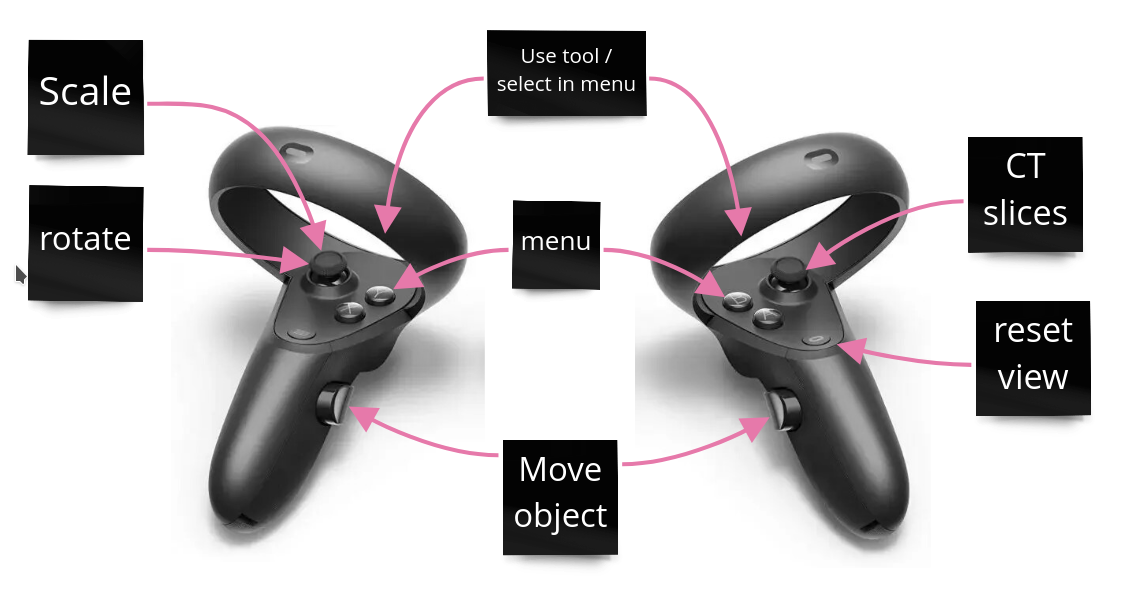
\includegraphics[height=120pt]{images/controllers.png}}
	\hfill
  \caption{Keybindings on Quest controllers}
  \small
  This illustration is also used within the application.
\end{figure}

The most common operations are bound to trigger and grip button, which is easily reachable on most controllers. The controller trigger mimics a mouse click on a pc, and so it is used for clicking buttons and using selected tools. The grip button mimics a real-world grabbing gesture and is used for grabbing a model part.
The primary button is used for opening the menu.
For ease of use, the two controllers are mostly mirrored, except for the joystick. The right joystick is used for scrolling through CT slices, similar to how the scroll wheel is used in CT image viewers. The left joystick rotates and scales the entire model while keeping all the model parts correctly positioned.

\subsubsection{Menu system}
A menu system is implemented to allow the user to navigate less common operations while not distracting from inspecting the model.
When the menu button is pressed, the menu screen appears in front of the user. It is shown in world space, which means the text appears as a physical screen. The model is temporarily hidden to ensure the menu is always in the user's field of view. Placing content at the center of the screen avoids a typical VR UX problem where some information is not visible to the user.

\begin{figure}[h!]
    \centering
	\subfloat[][]{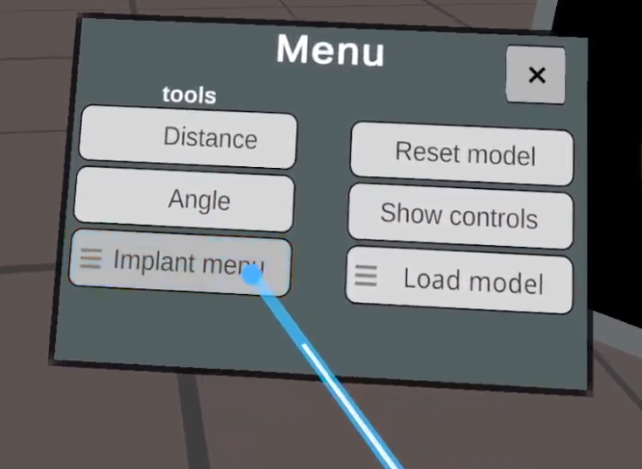
\includegraphics[height=120pt]{images/menu.png}}
	\hfill
  \caption{Menu screen}
  \small
  The main menu screen. The user is hovering one of the buttons.
~\cite{mishra_virtual_2019}

\end{figure}
The menu includes access to less frequent actions that do not require their own keybinding. The initial menu includes fast access to simple tools (e.g., measurement) and buttons to sub-menus. A hamburger menu icon suggests the button leads to a sub-menu.


\subsubsection{Measurements}
Some important functionality available in desktop VR viewers should also be available here. This includes measurement of distance and measurement of angles.
The measure tools works by selecting a start and an end point. The angle measurement additionally requires a middle point.
After placing the first point, a preview of the measurement result is shown as a line to give feedback to the user of the current state.
Using the outline shader mentioned before makes it possible to see the placed points even when obscured by the model, and the line between the points is always visible. This, combined with depth in VR makes it easy to understand where the points are placed and what the length and angle is.

\begin{figure}[h!]
    \centering
	\subfloat[][]{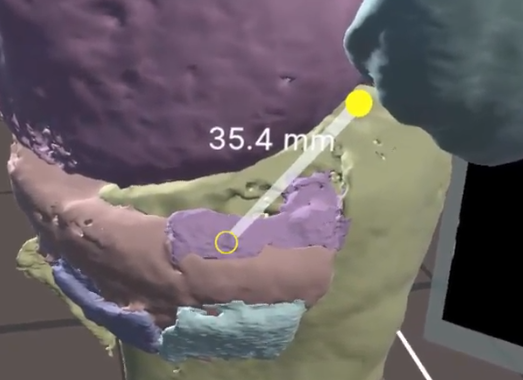
\includegraphics[height=120pt]{images/measure.png}}
	\hfill
  \caption{Distance measurement}
  \small
  A distance measurement. The yellow hollow circle is inside the model, and the filled circle is in front of the model.
~\cite{mishra_virtual_2019}
\end{figure}


\section{DICOM data visualisation}
I received several anonymized CT scan files from Helse Vest to use as input data. The CT scans are sent as DICOM packages\cite{noauthor_dicom_nodate}, where the scan is stored as several files, each representing a slice.
The model is also split up into bone fragments. The files include 3D surface models as STL files, where each file contains one bone. The STL files are created by (radiograf ???) at Haukeland University Hospital.

\subsection{Unity with custom file types}

To be able to read the DICOM files, the build produced by Unity needs access to the files. Unity has several built-in solutions to this.
The most common is the Resources functionality\cite{resourcesload_unity_nodate} that builds the application and includes all files in a `Resources' folder. Android projects are built in the standard APK format and also require special file paths and using the built-in web request to read files. This is not well documented, especially for the Quest, so this method was scrapped.

The easiest way of referencing files is usually setting a reference in the unity editor, and the file will be included in the build. This works great with common files like images, but Unity does not allow custom file types without 'hacking' the Unity inspector and creating a custom file importer\cite{scriptedimporters_unity_nodate}, that has lacking documentation. The solution to this is to rename all DICOM files to {name}.bytes. This makes Unity handle the files as 'TextAsset' text files\cite{textassets_unity_nodate}. I then open the files as text files and create a byte stream. The byte stream is then used for rendering with the DICOM library.

\subsection{Rendering CT image}

To render CT images from the DICOM data, I used the .NET library \emph{Fellow Oak DICOM}\cite{noauthor_fellow_2022}. It is an open-source library for parsing DICOM data and image rendering.
I use the data the DICOM files to create a $Slice$ object for each of the files. The slice object implements reading the density value at position $(x, y)$ at that slice. a Unity Texture is created for each slice to render the image in Unity.

Every pixel on the texture is set to the greyscale color correlating to the density value. To find the color in a position, calculate $(density-minDensity)/(maxDensity-minDensity)$. If result is 1, it has maximum density and is set to white color.

\begin{figure}[h!]
    \centering
	\subfloat[][]{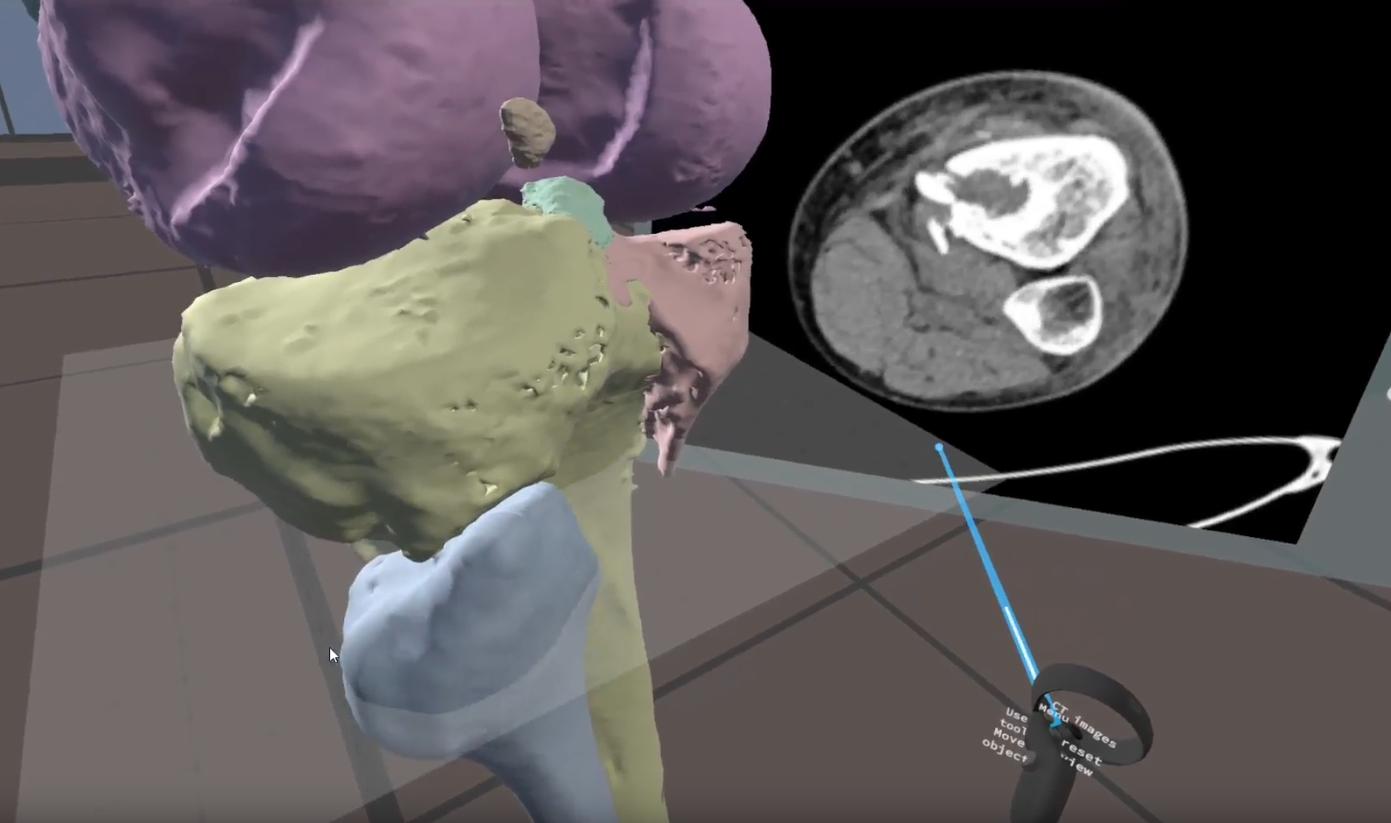
\includegraphics[height=120pt]{images/ctscan.png}}
	\hfill
  \caption{CT images}
  \small
  The user has moved the CT slice plane (transparent grey) to inspect the Tibia and Fibula (Shinbone/Calf Bone). The CT image on the right shows the CT scan of the two bones.
~\cite{mishra_virtual_2019}
\end{figure}


\subsection{Rendering intersection}
While rendering the selected slice as an image gave some understanding, there was still a disconnect between the model and the CT image. To improve upon this, I rendered the CT image at the exact position where it would intersect with the model.
This required removing the part of the model above/under the intersection plane, so it did not obscure the image. For this, I used a Unity Assetstore shader to view the cross-section of a mesh\cite{aldandarawy_unity_2019}.

This effect can be disturbing as the entire model is not visible. To allow for rendering the entire model, this rendering is a made optional. The option defaults to showing the entire model because it is easier to understand.
The toggle button is shown in the CT image options.


\section{tests}


\subsection{test 1}
date: 16 jan. 2022
This was the first test done with professional end users. The goal of the test was to figure out if any of the proposed use-cases was relevant for the user. The test was performed by introducing the software, its potential use-cases and a short introduction on how to use the VR controllers.
As both surgeons are very experienced with reading 2D CT images, they agreed that using 3D and VR to improve the understanding of fractures were minimal.

\begin{table}[ht]
\begin{tabular}{p{0.15\linewidth} |p{0.15\linewidth} |p{0.15\linewidth} | p{0.5\linewidth}}
Occupation         & Experience & proficiency with VR & comments                                                                                                                                \\hline
Orthopedic surgeon & 10+ years  & None                & The density of bone is important to know parts are solid enough for drilling. Also, some parts below the desnity threshold are missing. \\
Orthopedic surgeon & 10+ years  & None                & Smaller parts and bone fragments should be moveable to "reponere bruddet".                                                              \\
                   &            &                     &
\end{tabular}
\end{table}

The tests are generally well received but there are still no conclusion on the research questions.



%\bibliographystyle{splncs04}
%\bibliography{references}
\printbibliography

\end{document}
